\subsection{Saddlepoint approximation} \label{sec-saddlepoint}

This section presents another approximation scheme based on the Edgeworth approximation, which resolves some of the issues of the Edgeworth approximation highlighted in the previous section.

We begin by introducing \textit{exponential tilting}. Consider a random variable $X \in \Rp$ with cumulant generative function $K$ and density $f$. We introduce the exponential family $\mathcal{T}_P = \{ P_\gamma \}_{\gamma \in \Rp}$ where each $P_\gamma \in \mathcal{T}_P$ is characterized by its density function $f(\cdot; \gamma)$ given by
\begin{equation*}
    f(x; \gamma) = f(x)\expf{\gamma^\top x - K(\gamma)}.
\end{equation*}
Note that by the definition of the cumulant generating function, $K(\gamma)$ is the right normalization factor for $f(\cdot; \gamma)$ to integrate to 1, and hence $f(\cdot; \gamma)$ is a valid density function. Furthermore, the original distribution $P$ is an element of $\mathcal{T}_P$ with $P = P_0$. Given two distributions $P_{\gamma_0}, P_\gamma \in \mathcal{T}_P$, their densities differ by a known factor
\begin{equation*}
    f(x; \gamma_0) = f(x; \gamma)\expf{(\gamma_0 - \gamma)^\top x - \left[K(\gamma_0) - K(\gamma)\right]}.
\end{equation*} 
Hence, choosing $\gamma_0 = 0$ gives $f(\cdot; \gamma_0) = f$ and the following holds for any $\gamma \in \Rp$
\begin{equation} \label{eq-saddlepoint-original}
    f(x) = f(x; \gamma)\expf{K(\gamma) - \gamma^\top x}.
\end{equation}
Therefore, we can construct an approximation of $f$ by choosing $\gamma$ such that $f(\cdot; \gamma)$ can be accurately approximated.

Let us now consider a distribution $P$ with cumulant generating function $K$. We wish to use the previous argumentation to approximate the density $f_n$ of the mean $S$ of $n$ i.i.d.\,random variables distributed according to $P$. Using that the cumulant generating function of $S$ is $K_n(t) = nK(t/n)$ and replacing it in (\ref{eq-saddlepoint-original}), we get
\begin{equation} \label{eq-fn-in-terms-of-fngamma}
    f_n(s) = f_n(s; \gamma)\expf{nK(\gamma / n) - \gamma^\top s},
\end{equation}
where $f_n(\cdot; \gamma)$ is the density of the mean of $n$ i.i.d.\,random variables distributed according to $P_\gamma$. Since the Edgeworth approximation was derived for a standardized sum of random variables, we apply the transformation
\begin{align*}
    \frac{1}{n}\sum_{i=1}^n X_i &\mapsto \frac{1}{\sqrt{n}}\sum_{i=1}^n \Sigma_\gamma^{-1/2}(X_i - \mu_\gamma)\\
    s &\mapsto s^* := \sqrt{n}\Sigma_\gamma^{-1/2}(s - \mu_\gamma)
\end{align*}
where $\mu_\gamma$ and respectively $\Sigma_\gamma$ are the mean and covariance under the distribution $P_\gamma$. Furthermore, the determinant of the transformation is $n^{p/2}|\Sigma_\gamma|^{-1/2}$, which gives, using the notation in (\ref{eq-edge-polynomial}),
\begin{equation} \label{eq-saddlepoint-poly}
    f_n(s; \gamma) = n^{p/2}|\Sigma_\gamma|^{-1/2} \phi(s^*)\left\{ 1 + P_{k, n}(s^*; \kappa(\gamma)) + o(n^{1-k/2})\right\},
\end{equation}
where $\kappa(\gamma)$ are the cumulants of the random variable distributed according to $P_\gamma$. The cumulant generating function $K(\cdot; \gamma)$ of $P_\gamma$ can be expressed in terms of the cumulant generating function $K$ by
\begin{equation*}
    K(t; \gamma) = K(t + \gamma) - K(\gamma).
\end{equation*}
Since the covariance matrix $\Sigma_\gamma$ is equal to the Hessian of the cumulant generating function $K(\cdot; \gamma)$ of $P_\gamma$ evaluated at 0, we have $\Sigma_\gamma = K''(\gamma)$. This lets us rewrite (\ref{eq-saddlepoint-poly}) in terms of $K$ as follows,
\begin{equation*}
    f_n(s; \gamma) = n^{p/2}|K''(\gamma)|^{-1/2} \phi(s^*)\left\{ 1 + P_{k, n}(s^*; \kappa(\gamma)) + o(n^{1-k/2})\right\}.
\end{equation*}

We are now interested in choosing $\gamma$ such that the Edgeworth approximation of $f_n(\cdot; \gamma)$ is accurate. As seen in Remark \ref{rem-edge-mean}, the Edgeworth approximations of even order $k$ have an approximation error of $O(n^{-k/2})$ instead of $o(n^{1-k/2})$ when evaluated at the mean of the distribution. In other words, the Edgeworth approximation will be more accurate if $s^* = 0$ in the previous equation. Since $\gamma$ can be chosen freely and differently for each value $s$ at which the density $f_n$ is evaluated, we can choose $\gamma$ such that $s^* = 0$, or equivalently, such that $s = \mu_\gamma$. Similarly to the covariance matrix, we can write the mean of $P_\gamma$ as $\mu_\gamma = K'(\gamma)$. Hence, for any $s \in \Rp$, we find a distribution $P_{\hat\gamma_s} \in \mathcal{T}_P$ with mean $s$ by solving
\begin{equation} \label{eq-saddlepoint}
    K'(\hat\gamma_s) = s.
\end{equation}
We call the solution of this equation $\hat\gamma_s$ to emphasize the fact for each $s \in \Rp$, a different tilting distribution $P_{\hat\gamma_s}$ is chosen such that the Edgeworth approximation to the density of $P_{\hat\gamma_s}$ is accurate in $s$. Note that if $\hat\gamma_s$ solves (\ref{eq-saddlepoint}), it is also the maximum likelihood estimator of $\gamma$ within the model $\mathcal{T}_P$. Replacing $\gamma$ by $\hat\gamma_{s}$ in (\ref{eq-saddlepoint-poly}), we get
\begin{equation*}
    f_n(s; \hat\gamma_s) = \left(\frac{n}{2\pi}\right)^{p/2}|\Sigma_{\hat\gamma_s}|^{-1/2}\left\{ 1 + P_{k, n}(0; \kappa(\hat\gamma_s)) + O(n^{-k/2})\right\}.
\end{equation*}
Replacing $f_n(s; \gamma)$ by the approximation above in (\ref{eq-fn-in-terms-of-fngamma}) gives
\begin{align}
    f_n(s) &= \left(\frac{n}{2\pi}\right)^{p/2} \frac{\expf{nK(\hat\gamma_s / n) - \hat\gamma_s^\top s}}{|K''(\hat\gamma_s)|^{1/2}}  \left[1 + P_{k, n}(0; \kappa(\hat\gamma_s)) + O(n^{-k/2})\right]\nonumber\\
    &= g(s; K)\left[1 + P_{k, n}(0; \kappa(\hat\gamma_s)) + O(n^{-k/2})\right] \label{eq-saddle-exp}
\end{align}
where
\begin{equation*}
    g(s; K) = \left(\frac{n}{2\pi}\right)^{p/2} \frac{\expf{nK(\hat\gamma_s / n) - \hat\gamma_s^\top s}}{|K''(\hat\gamma_s)|^{1/2}}.
\end{equation*}
We call $g(\cdot; K)$ the \textit{Saddlepoint approximation} to the density of $S$. We now justify the approximation accuracy claim from (\ref{eq-saddle-exp}) in the following theorem.

\begin{theorem}
    Let $P$ be a distribution with cumulant generating function $K$ and $k \in \N_{\geq 2}$ such that all cumulants of $P$ of order up to $k$ exist. Suppose that for every $s \in \Rp$, (\ref{eq-saddlepoint}) has a unique solution $\hat\gamma_s$. Let $n \in \N$ let $S$ be the mean of $X_1, \ldots, X_n \simiid P$,
    \begin{equation*}
        S = n^{-1} \sum_{i=1}^n X_i.
    \end{equation*}
    Then, if the density $f_n$ of $S$ exists, the expansion given in (\ref{eq-saddle-exp}) holds.
\end{theorem}
\begin{proof}
    This result is a direct consequence of Theorem \ref{thm-edgeworth}, applied pointwise to the tilted distribution $P_{\hat\gamma_s}$ for every $s \in \Rp$. As discussed above, Remark \ref{rem-edge-mean} implies that only powers of $n^{-1}$ have non-vanishing coefficients in the Edgeworth approximation of the tilted densities. This turn implies that the Edgeworth approximation error in each point is of order $O(n^{-k/2})$, concluding the proof of the theorem.
\end{proof}

While the Saddlepoint approximation has many advantages over the Edgeworth approximation, it is important to note that the Saddlepoint approximation requires the complete cumulant generating function of the approximated density to be known. The Edgeworth approximation on the other hand only uses the first $k$ cumulants of the distributions, which are evaluations of derivatives of the cumulant generating function in 0. 

A special case of particular interest arrises when taking $k = 2$. In this case, the Edgeworth approximation of $f_n(\cdot; \hat\gamma_s)$ is equal to its normal approximation since the polynomial part $P_{k, n}(\cdot; \kappa(\hat\gamma_s))$ of $e_{k,n}(\cdot; \kappa(\hat\gamma_s))$ is equal to 0, giving
\begin{align} \label{eq-saddle-3}
    f_n(s) &= g(s; K)\left[1 + O(n^{-1})\right]\nonumber\\
    &= \left(\frac{n}{2\pi}\right)^{p/2} \frac{\expf{nK(\hat\gamma_s / n) - \hat\gamma_s^\top s}}{|K''(\hat\gamma_s)|^{1/2}} \left[1 + O(n^{-1}))\right]
\end{align}
The Saddlepoint approximation of second order is commonly used in applications since it presents many advantages compared to the Edgeworth approximation. It has a simple expression which makes it easier to construct and manipulate it. Furthermore, the Saddlepoint approximation is often highly accurate or even exact up to normalization, and, unlike the other approximations presented so far, it is always positive.

\begin{example} \label{ex-gamma-saddle}
    Extending Example \ref{ex-gamma-edge}, we analyze the behaviour of the Saddlepoint approximation to the mean $Y = n^{-1}\sum_{i=1}^n X_i \in \R_+$ where $X_1, \ldots, X_n \simiid \Gamma(p, \lambda)$. The cumulant generating function of the $\Gamma(n, p)$ distribution is $K(t) = p\logf{\lambda} - p\logf{\lambda - t}$ and its first derivative is $K'(t) = p / (\lambda - t)$. For any $s \in \R_+$, the Saddlepoint $\hat\gamma_s$ is given by the solution to the Saddlepoint Equation in (\ref{eq-saddlepoint}), which here becomes
    \begin{equation*}
        \frac{p}{\lambda - \hat\gamma_s/n} = s \Rightarrow \hat\gamma_s = n\left(\lambda - \frac{p}{s}\right).
    \end{equation*}

    \begin{figure}[!htbp]
        \textbf{Approximation error of $\Gamma(2,1)$ standardized sums with $n=10$}
        \centering
        \subfloat{
            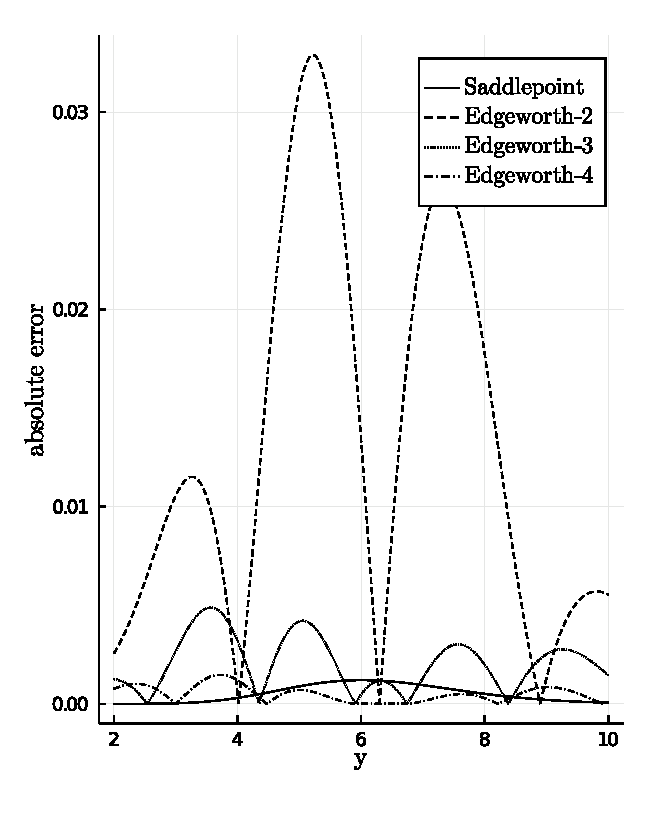
\includegraphics[width=7.5cm]{saddlepoint_and_edgeworth_err_abs_gamma21_10_terms.eps} 
        }
        \subfloat{
            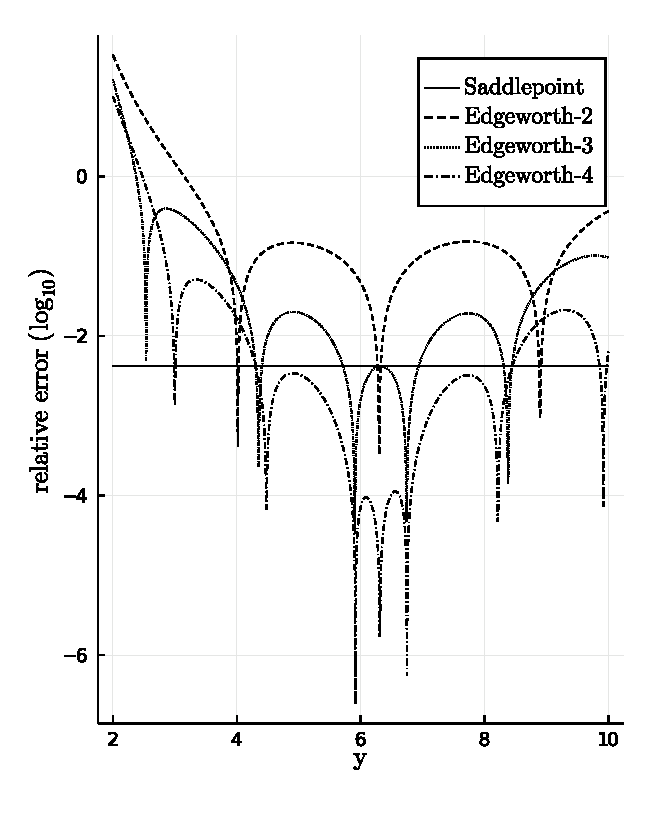
\includegraphics[width=7.5cm]{saddlepoint_and_edgeworth_err_rel_gamma21_10_terms.eps} 
        }
        \caption{Study of the error of the Saddlepoint approximation on a standardized sum $n=10$ i.i.d.\,random variables distributed according to $\Gamma(2, 1)$. Both panes demonstrate the properties studied of the Saddlepoint approximation: the accurate relative error, the gain in order of approximation and the uniform relative error of the approximation for sums of Gamma random variables.}
        \label{fig-saddlepoint-err}
    \end{figure}

    In Figure \ref{fig-saddlepoint-err}, we demonstrate how the Saddlepoint approximation of second order compares to the Edgeworth approximation when approximating a standardized sum of $n$ random variables independently distributed according to $\Gamma(2, 1)$. Since the standardized sum can be obtained by multiplying the mean by a factor of $\sqrt{n}$, the Saddlepoint approximation is easily adapted by change of variable. Both panels show accurate approximation properties both in terms of relative and absolute error.
    \newline
    In this example, it is also interesting to examine the explicit form of the Saddlepoint approximation $g$. Replacing the relevant quantities in (\ref{eq-saddle-3}), we obtain that the Saddlepoint approximation is
    \begin{align*}
        g(s; K) &= \sqrt{\frac{n}{2\pi K''(\lambda - \frac{p}{s})}} \expf{nK\left(\lambda - \frac{p}{s}\right) - n\left(\lambda - \frac{p}{s}\right)s}\\
        &= \sqrt{\frac{n}{2\pi s^2/p}} \expf{n\left(p\logf{\lambda} - p\logf{p/s}\right) - ns\lambda + np}\\
        &= (n\lambda)^{np}s^{np-1}\expf{-sn\lambda}  \frac{(np)^{1/2-np}\expf{np}}{\sqrt{2\pi}}.
    \end{align*}
    Consider now Stirling's formula for the gamma function
    \begin{equation*}
        \Gamma(z) \approx \sqrt{2\pi}z^{z-1/2}\expf{-z}.
    \end{equation*}
    We recognize that the second term in the expression of $g(s; K)$ corresponds to the inverse of Stirling's approximation of $\Gamma(np)$. Therefore, the Saddlepoint approximation to the density of the mean $n$ i.i.d.\,random variables distributed according to $\Gamma(p, \lambda)$ corresponds to the density of the true distribution $\Gamma(np, n\lambda)$ of the mean, where the gamma function has been replaced by Stirling's approximation. This has the interesting consequence that the relative error of the Saddlepoint approximation does not depend on $s$, the point at which the density is evaluated, but rather only depends on $n$. This behaviour is also seen in Figure \ref{fig-saddlepoint-err} where the relative error of the Saddlepoint approximation is a straight horizontal line. Daniels \cite{daniels1954saddlepoint} characterizes the class of distributions for which the uniform relative approximation error holds.

  
    
\end{example}